
\documentclass[a4paper,12pt,twoside]{article}
\usepackage[a4paper,top=20mm,bottom=20mm,inner=38mm,outer=19mm]{geometry}
\usepackage{graphicx}
\usepackage{float}
\usepackage{url}
\usepackage{listings}
\usepackage{subfigure}
\usepackage{cite}
\usepackage{amssymb}
\usepackage{parskip}
\usepackage{setspace}
\bibliographystyle{apalike} 
\begin{document}
\onehalfspacing

\begin{titlepage}
\clearpage
\vspace*{\fill}
\begin{center}
\begin{minipage}{.6\textwidth}
\centerline{\textbf{\huge Gathering Atmospheric Data}}
\centerline{\textbf{\large Using an Unmanned Air Vehicle}}
\centerline{\textit{Henry Miskin}}
\centerline{\textit{\today}}
\end{minipage}
\end{center}
\vspace{5cm}
\center
\textbf{Abstract}
\center
This report looks at three dimensional energy based path planning for unmanned air vehicles in a predetermined area, with particular consideration to quality of data produced.
\vfill

\clearpage
\end{titlepage}
\tableofcontents
\clearpage

\section{Introduction}
\label{sec:introduction}

The following section outline the process in which a minimum cost route through a sample space can be obtained that provides the best data collection quality

\section{Plane Properties}
\label{sec:plane_properties}

\begin{table}[width=\textwidth]
\centering
    \begin{tabular}{cc}
    Wingspan	& 3	\\
Turn Radius	& 0.1	\\

    \end{tabular}
\caption{Table of Plane Properties}
\label{tbl:table_of_plane_properties}
\end{table}

To considere th minimum cost of circumnavigating a particular route the specifications of a plane must be considered in table \ref{tbl:table_of_plane_properties} the plane detailed in this table is the plane that is used for the entire report

\section{Energy Model}
\label{sec:energy_model}

\begin{equation}
\label{eq:energy_equation}
E=\alpha D + \beta H
\end{equation}

From these plane properties the following energy model has been definened in equation \ref{eq:energy_equation} where $\alpha$ and $\beta$ are coeficients that are determined by the plane. For the current plane shown in table \ref{tbl:table_of_plane_properties} $\alpha$ and $\beta$ take values of 10 and 6 respectively.

\section{Latin Hypercubes}
\label{sec:latin_hypercubes}

Latin hypercubes are sampling pland that provide the best space fillingness while limiting the total number of sampling points required. This is generally applied to testing of computer similations where the collection of each point is expensive. In this situation however the travel bertween the points the expensive component.

\begin{figure}[H]
	\centering
	
	\subfigure[10 Nodes]{
		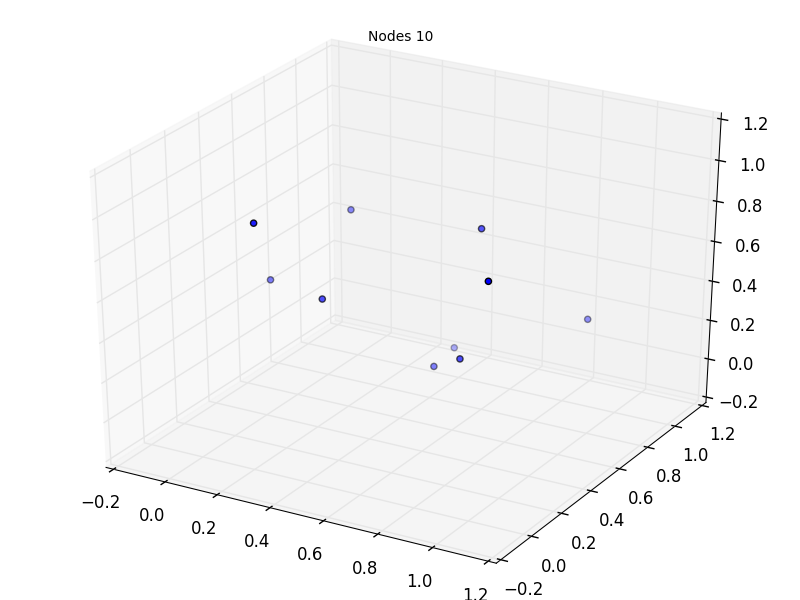
\includegraphics[width=0.4\textwidth]{figures/nodes_10.png} 
		\label{fig:10_nodes}
	}
	\subfigure[25 Nodes]{
		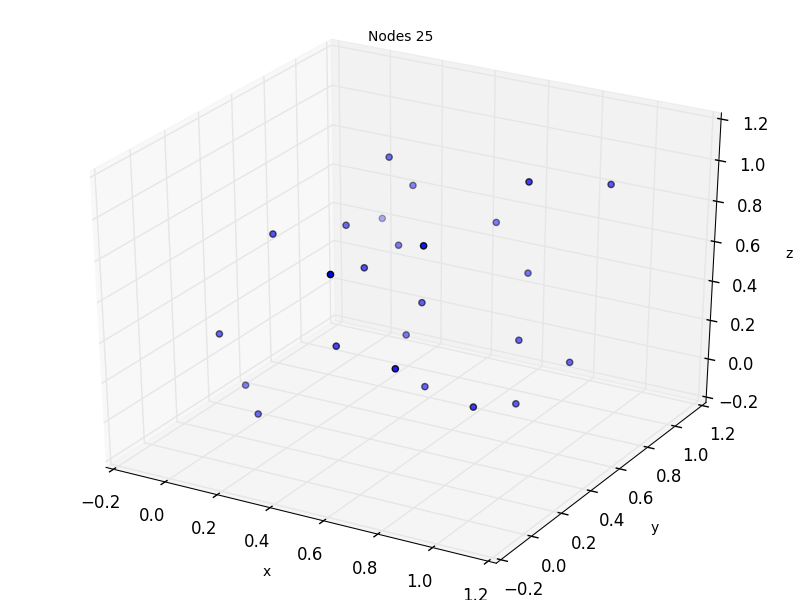
\includegraphics[width=0.4\textwidth]{figures/nodes_25.png} 
		\label{fig:25_nodes}
	}
	\subfigure[50 Nodes]{
		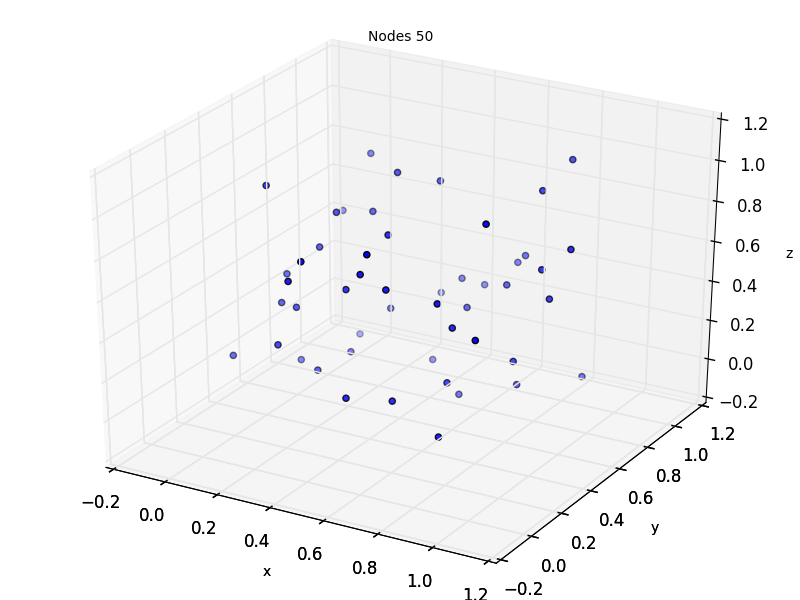
\includegraphics[width=0.4\textwidth]{figures/nodes_50.png} 
		\label{fig:50_nodes}
	}
	\subfigure[100 Nodes]{
		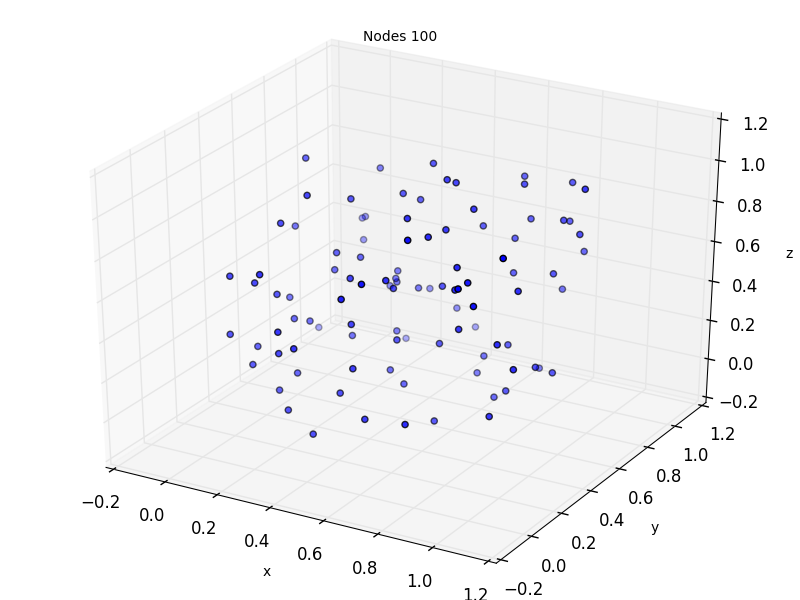
\includegraphics[width=0.4\textwidth]{figures/nodes_100.png} 
		\label{fig:100_nodes}
	}
	\caption{Latin Hypercubes with Varying Numbers of Nodes}
	\label{fig:latin_hypercubes_with_varying_numbers_of_nodes}
\end{figure}

Figure \ref{fig:latin_hypercubes_with_varying_numbers_of_nodes} shows a number of latin hypercubes with differnt numbers of nodes. All the Latin Hypercubes are within a unit cube. For collection of data in a required area these cubes can be stretched to fill the desired space. This does not provide an even spacing in each direction however means that eeach vertex of data collection is equally considered.

For this project the idea is to follow this logic to utilise Latin Hypercubes:

\begin{enumerate}
\item Specifiy area of interest to researcher
\item Estimate number of nodes able to be circumnavigated given the UAV total energy and the area of sample space
\item Fit Latin Hypercube of given nodes to sample area
\item Calcualte least energy route through the sample space
\item After first flight asses areas of encertainty to plan route through for next flight

\end{enumerate}

\section{Route Planning}
\label{sec:route_planning}

Given a set of points within a sample space the next stage of the proceedings is to compute the least cost route through these points. This problem presents itself in the forn of the travelling salesman problem. The travelling salesman problem is the problem of finding the least cost route through a set of points. There is lots of work done on the elicidean travelling salesman problem and introducing heroustics to improe the time taken to compute. This is due to the problem being an NP hard problem (the computing time required increases exponentially with the number of points in the route)

\subsection{Exact Travelling Salesman}
\label{sec:exact_travelling_salesman}

\begin{figure}[H]
	\centering
	
	\subfigure[4 Nodes]{
		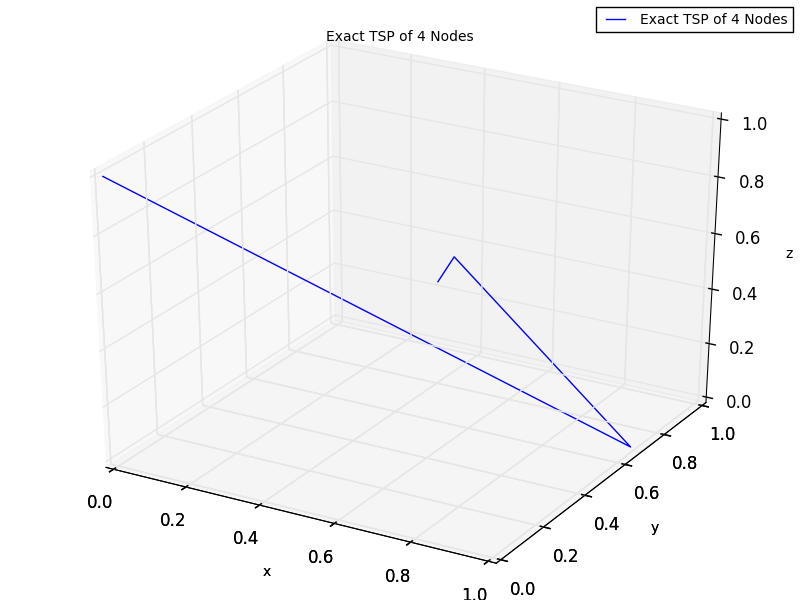
\includegraphics[width=0.4\textwidth]{figures/exact_tsp_of_4_nodes.png} 
		\label{fig:4_nodes}
	}
	\subfigure[6 Nodes]{
		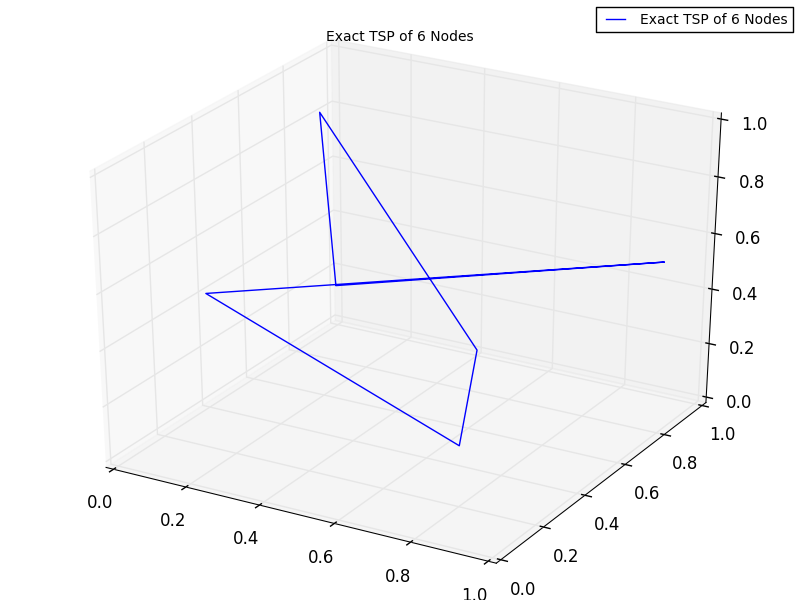
\includegraphics[width=0.4\textwidth]{figures/exact_tsp_of_6_nodes.png} 
		\label{fig:6_nodes}
	}
	\subfigure[8 Nodes]{
		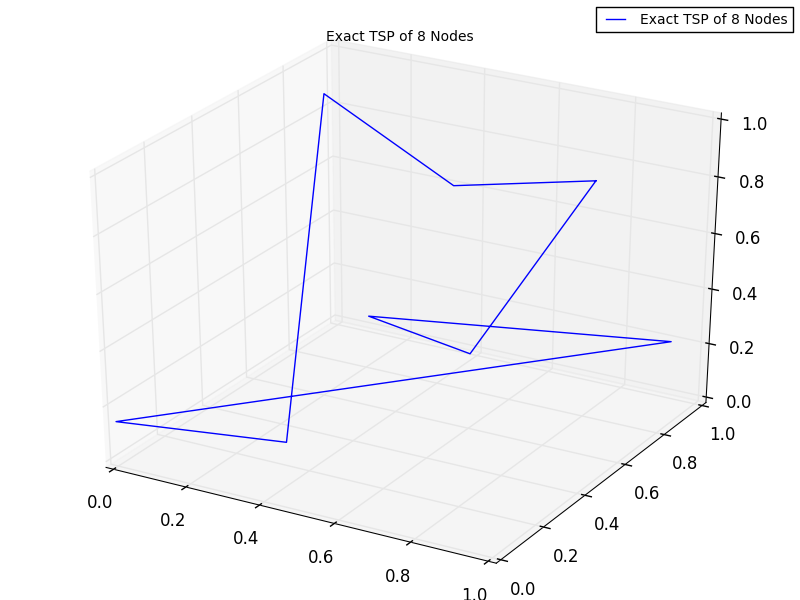
\includegraphics[width=0.4\textwidth]{figures/exact_tsp_of_8_nodes.png} 
		\label{fig:8_nodes}
	}
	\subfigure[10 Nodes]{
		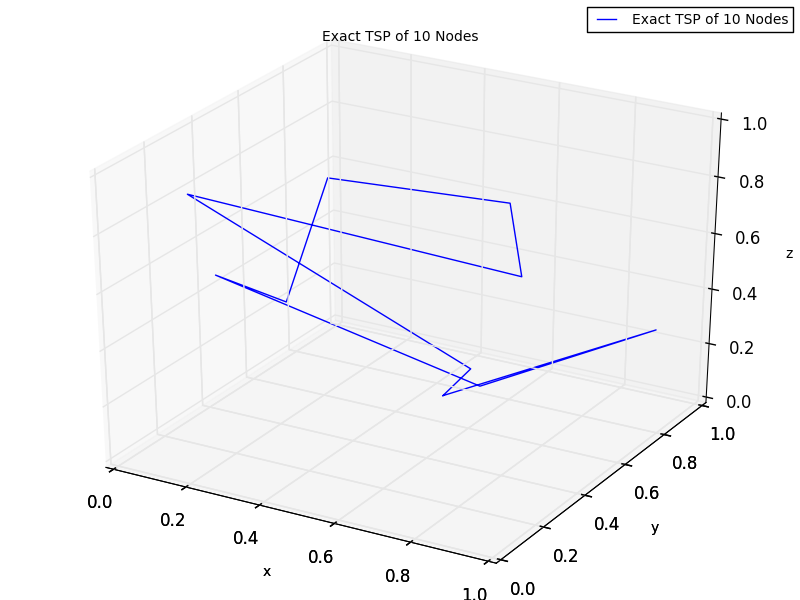
\includegraphics[width=0.4\textwidth]{figures/exact_tsp_of_10_nodes.png} 
		\label{fig:10_nodes}
	}
	\caption{Exact routes calculated by travelling salesman}
	\label{fig:exact_routes_calculated_by_travelling_salesman}
\end{figure}

Figure \ref{fig:exact_routes_calculated_by_travelling_salesman} shows the optimal routes for differnt numbers of nodes. These optimal routes are found by computing the exact cost of each and every route option. Although this yield the shortest routes this approach is not efficient in terms of the computation time required.

\begin{table}[width=\textwidth]
\centering
    \begin{tabular}{lllll}
    Number of points	& 4	& 6	& 8	& 10	\\
Number of possible routes	& 24	& 720	& 40320	& 3628800	\\
Computation time (ms)	& 1.0	& 5.0	& 315.0	& 33267.0	\\
Best route cost (J)	& 110.38	& 106.71	& 106.72	& 108.76	\\

    \end{tabular}
\caption{Comparison of route calculation}
\label{tbl:comparison_of_route_calculation}
\end{table}

Table \ref{tbl:comparison_of_route_calculation} shows the number of possible routes and the resulting computation time given different numbers of nodes. It can easily be seen that the number of route options is equivilent to $n!$ where $n$ is the number of nodes. The number of routes directly realtes to the computation time.

The computation time of the exact TSP approach can be reduced in a number of ways. Primarily the start node of the calculation can be defined however this only reduces the complexity to the equivilent of removoing a node form the computation. Other approaches involve producing a best guess and improving upon that. The approach taken in this project is taken from considering the best routes in figure \ref{fig:exact_routes_calculated_by_travelling_salesman} generally comprise of a climbing component and a decending component.

\subsection{Improving Travelling Salesman}
\label{sec:improving_travelling_salesman}

The progressive travelling salesman is an approach to computing a best guess route for the least energy route for a number of points. The computation process is as follows

\begin{enumerate}
\item Order the nodes by there vertical location from lowest to highest
\item Considering the lowest N nodes compute all posible combinations to produce two routes from the given nodes
\item Compare all permutations of routes to return the least cost combination
\item Add first nodes of both routes to final route
\item Consider lowest N nodes that are not in the final route and reitterate
\item Work through all nodes until no nodes are left without a route

\end{enumerate}

\begin{table}[width=\textwidth]
\centering
    \begin{tabular}{lllll}
    Nodes in each route	& 2	& 3	& 4	& 5	\\
Computation time (ms)	& 2.0	& 3.0	& 52.0	& 4091.0	\\
Best route cost (J)	& 120.49	& 115.48	& 115.48	& 114.79	\\

    \end{tabular}
\caption{Comparison of route calculation}
\label{tbl:comparison_of_route_calculation}
\end{table}

Table \ref{tbl:comparison_of_route_calculation} shows the varying computation time for routes through a 10 node latin hypercube that have a differnet numbers of nodes in each route. This refers to the number of nodes that are consideered in each progressive itteration of the code.

\begin{figure}[H]
\centering
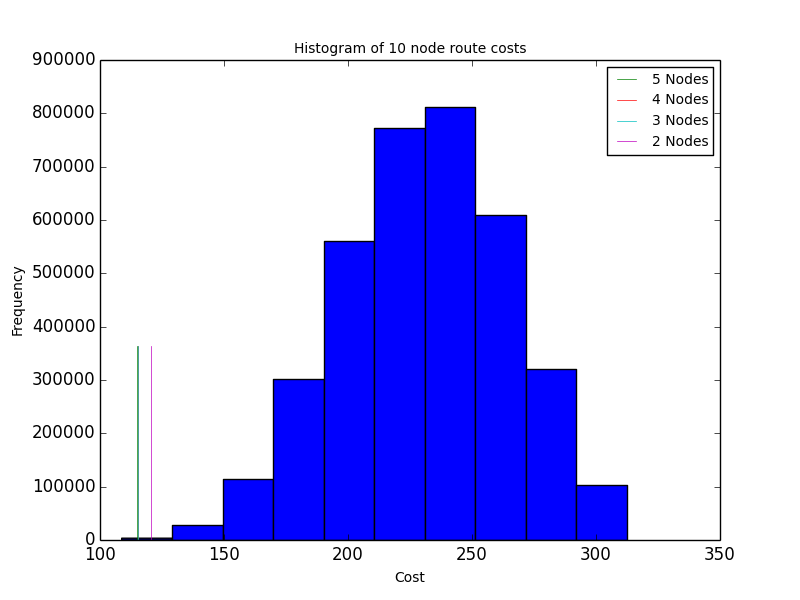
\includegraphics[width=0.8\textwidth]{figures/histogram_of_10_node_route_costs.png} 
\caption{Histogram of 10 node route costs}
\label{fig:histogram_of_10_node_route_costs}
\end{figure}

Figure \ref{fig:histogram_of_10_node_route_costs} shows a histogram of differnt route costs for a 10 node latin hypercube. The lines on this histogram plot represent the best cost routes with different numbers of nodes in the route

\subsection{Progressive Travelling Salesman}
\label{sec:progressive_travelling_salesman}

In section \ref{sec:progressive_travelling_salesman} a best guess approach to the travelling salesman was presented and compared with the exact results. Given the results were close to the optimum even when the progressive algorithem only considered 2 nodes in the route it can be brought forward to be considered in reference to larger route problems. In these routes 4 nodes are considered for both the up route and the down route are used at each stage of the progressive algorithm.

\begin{figure}[H]
	\centering
	
	\subfigure[10 Nodes]{
		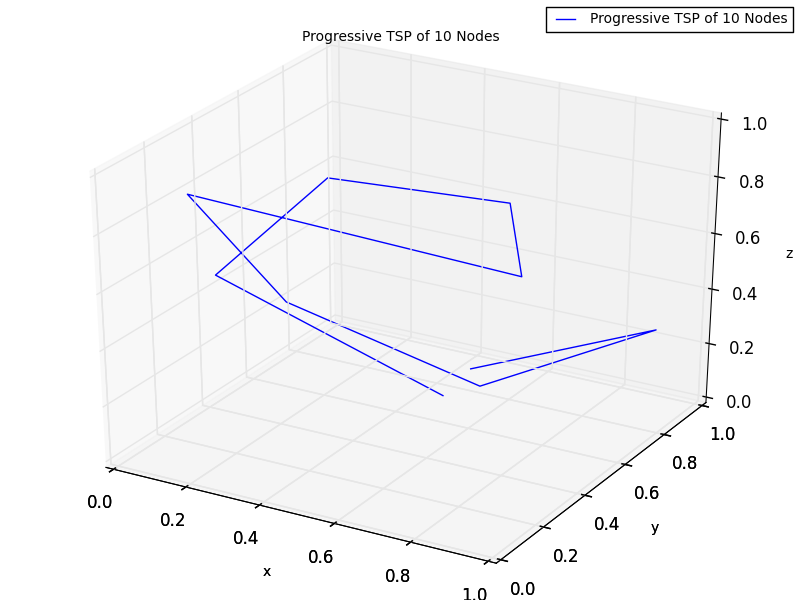
\includegraphics[width=0.4\textwidth]{figures/progressive_tsp_of_10_nodes.png} 
		\label{fig:10_nodes}
	}
	\subfigure[25 Nodes]{
		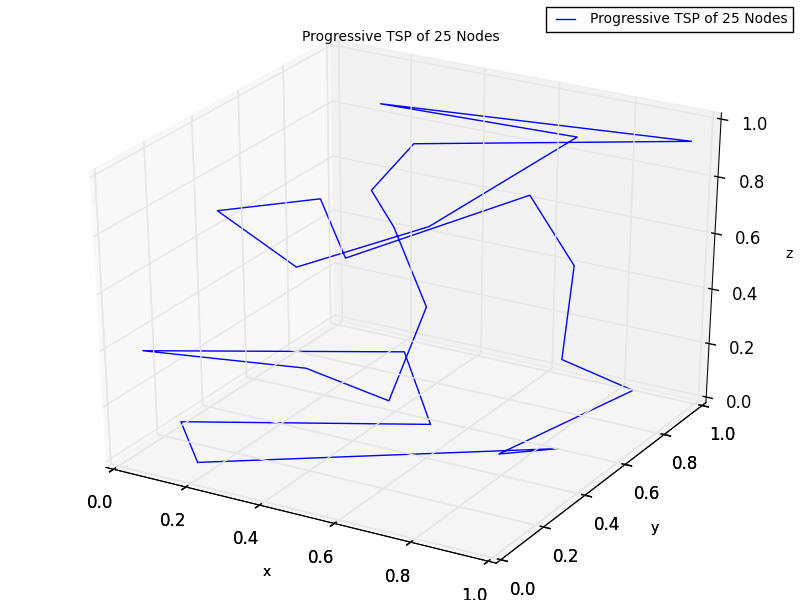
\includegraphics[width=0.4\textwidth]{figures/progressive_tsp_of_25_nodes.png} 
		\label{fig:25_nodes}
	}
	\subfigure[50 Nodes]{
		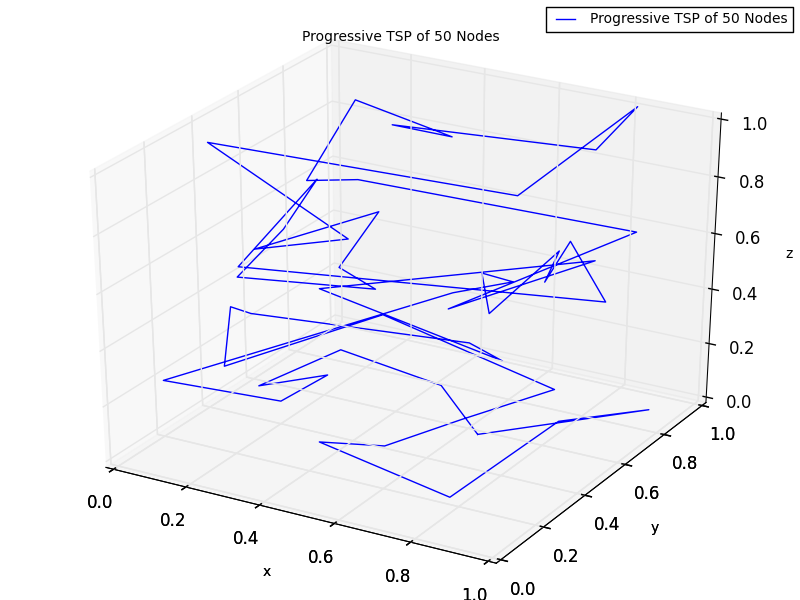
\includegraphics[width=0.4\textwidth]{figures/progressive_tsp_of_50_nodes.png} 
		\label{fig:50_nodes}
	}
	\subfigure[100 Nodes]{
		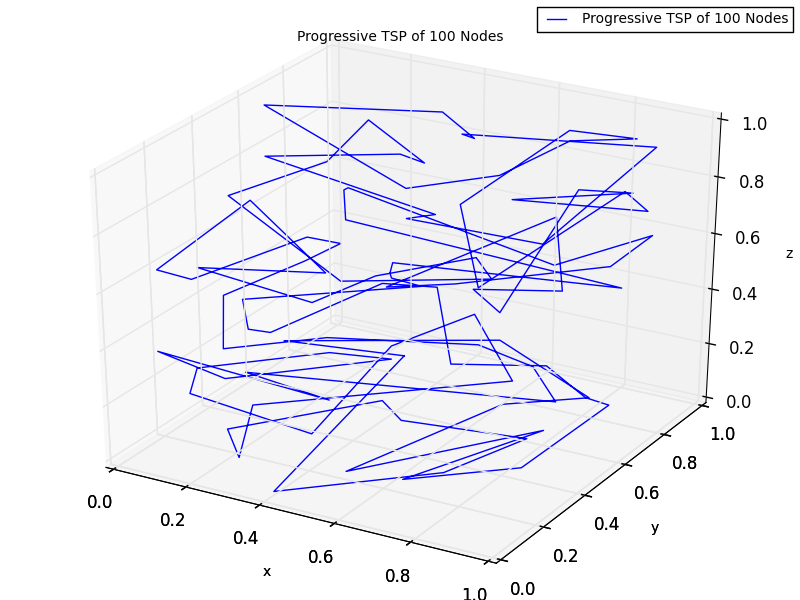
\includegraphics[width=0.4\textwidth]{figures/progressive_tsp_of_100_nodes.png} 
		\label{fig:100_nodes}
	}
	\caption{Exact routes calculated by travelling salesman}
	\label{fig:exact_routes_calculated_by_travelling_salesman}
\end{figure}

Figure \ref{fig:exact_routes_calculated_by_travelling_salesman} shows a number of optimal routes for varing numbers of nodes whos order is defined be the progressive travelling salesman algorithm. Though the 100 node route is difficult to see the exact routing the other routes show a logical approach to the routing problem

\begin{table}[width=\textwidth]
\centering
    \begin{tabular}{lllll}
    Number of points	& 10	& 25	& 50	& 100	\\
Computation time (ms)	& 52.0	& 236.0	& 591.0	& 1330.0	\\
Best route cost (J)	& 115.48	& 143.62	& 202.65	& 333.73	\\

    \end{tabular}
\caption{Comparison of progressive route calculation}
\label{tbl:comparison_of_progressive_route_calculation}
\end{table}

Table \ref{tbl:comparison_of_progressive_route_calculation} shows the computation time and route cost for the differnt routing situations. The computation time is far bellow that of the exact travelling salesman algorithm due to the complexity of this problem being broken down into 4 node chunks

\section{Path Planning}
\label{sec:path_planning}

The least energy route through a number of nodes has been defined however this route assumes that the UAV is able to turn on the spot and is not constricted by turning radius. Therefore to compute the actual energy cost of circumnavigating a route the turning radius of the UAV needs to be considered. Dubins paths are the minimum distance paths given a start and end direction.

Duibins paths ar comprised of maximum rate turns and straight line segments. The following defines all the routes that are possible made op of maxiumum rate turns and straight line segments

\begin{itemize}
\item RSR - Right Turn, Straight Flight then Right Turn
\item RSL - Right Turn, Straight Flight then Left Turn
\item LSR - Left Turn, Straight Flight then Right Turn
\item LSL - Left Turn, Straight Flight then Left Turn
\item RLR - Right Turn, Left Turn then Right Turn
\item LRL - Left Turn, Right Turn then Left Turn

\end{itemize}

\begin{figure}[H]
\centering
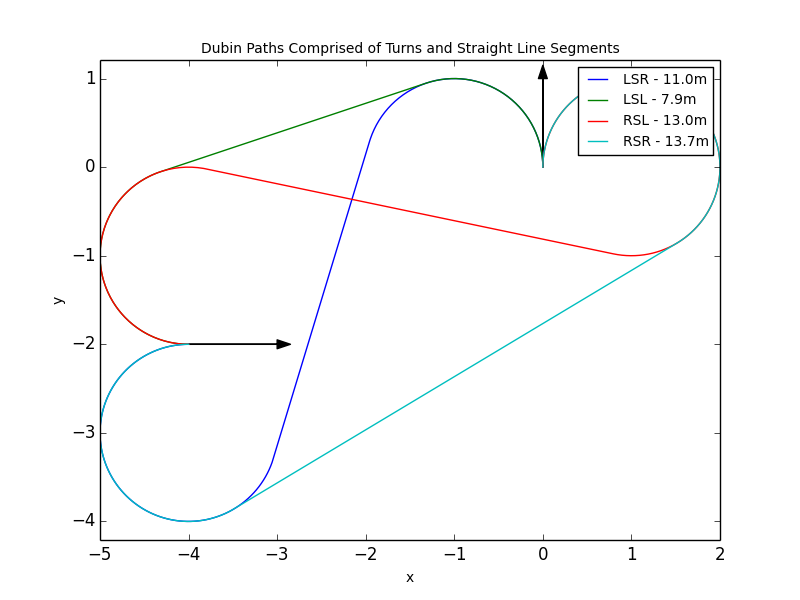
\includegraphics[width=0.8\textwidth]{figures/dubin_paths_comprised_of_turns_and_straight_line_segments.png} 
\caption{Dubin Paths Comprised of Turns and Straight Line Segments}
\label{fig:dubin_paths_comprised_of_turns_and_straight_line_segments}
\end{figure}

Figure \ref{fig:dubin_paths_comprised_of_turns_and_straight_line_segments} shows the possible routes from the point (0, 0) in direction (0, 1) to the point (-4, -2) in direction (1, 0). The arrows symbolise the start and end headings and the different coloured route symbolise the different routes. In this example the routes comprise of maximum rate turns of radius 1 and straight line segment. At close proximity these routes are not always possible

\begin{figure}[H]
\centering
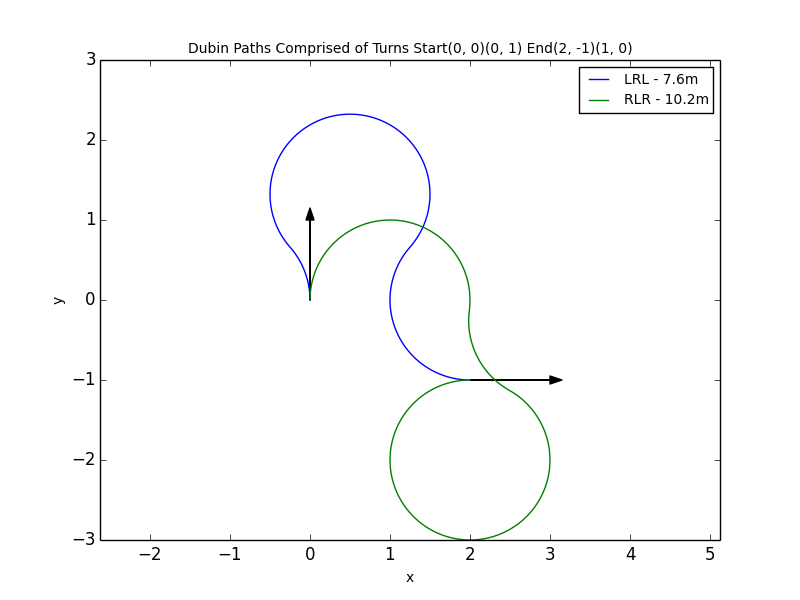
\includegraphics[width=0.8\textwidth]{figures/dubin_paths_comprised_of_turns_start(0,_0)(0,_1)_end(2,_-1)(1,_0).png} 
\caption{Dubin Paths Comprised of Turns Start(0, 0)(0, 1) End(2, -1)(1, 0)}
\label{fig:dubin_paths_comprised_of_turns_start(0,_0)(0,_1)_end(2,_-1)(1,_0)}
\end{figure}

Figure \ref{fig:dubin_paths_comprised_of_turns_and_straight_line_segments} shows the possible routes from the point (0, 0) in direction (0, 1) to the point (2, -1) in direction (1, 0). The arrows symbolise the start and end headings and the different coloured route symbolise the different routes. In this example the routes only comprise of maximum rate turns of radius 1. These routes are only viable when the distance between points is $D<4r$ where $D$ symbolises the distance.

\begin{figure}[H]
\centering
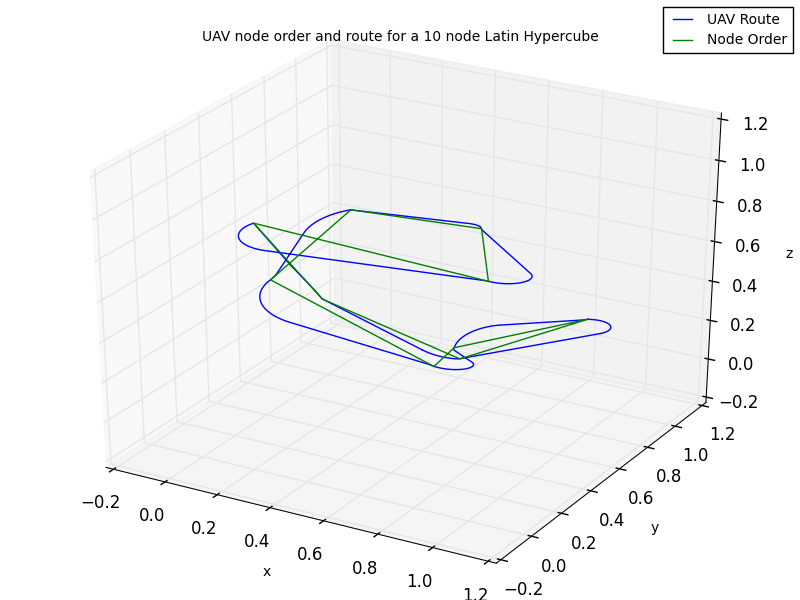
\includegraphics[width=0.8\textwidth]{figures/uav_node_order_and_route_for_a_10_node_latin_hypercube.png} 
\caption{UAV node order and route for a 10 node Latin Hypercube}
\label{fig:uav_node_order_and_route_for_a_10_node_latin_hypercube}
\end{figure}

Figure \ref{fig:uav_node_order_and_route_for_a_10_node_latin_hypercube} shows the optimal path and route for a UAV to circumnavigate a 10 node Latin Hypercube. The route is calculated before the path and then the path is calculated from the heading at each node in the route.

\begin{figure}[H]
\centering
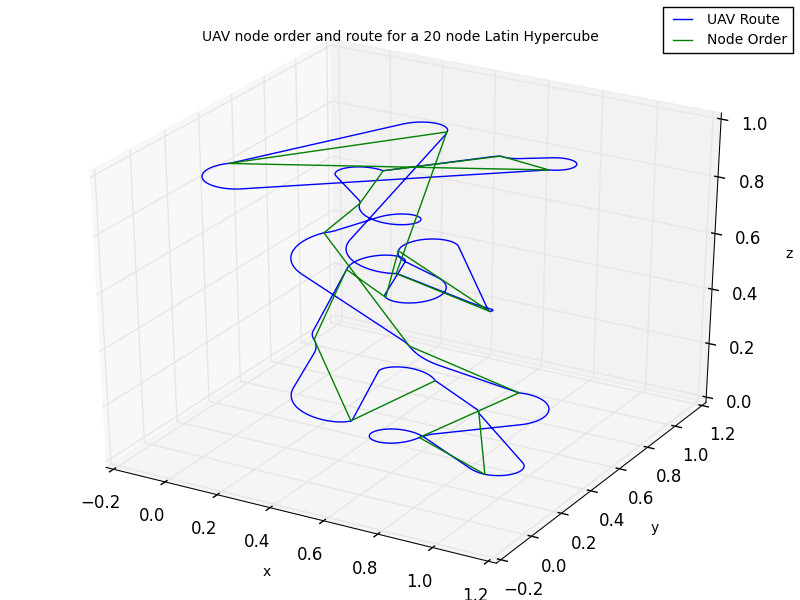
\includegraphics[width=0.8\textwidth]{figures/uav_node_order_and_route_for_a_20_node_latin_hypercube.png} 
\caption{UAV node order and route for a 20 node Latin Hypercube}
\label{fig:uav_node_order_and_route_for_a_20_node_latin_hypercube}
\end{figure}

Figure \ref{fig:uav_node_order_and_route_for_a_20_node_latin_hypercube} shows the optimal path and route for a UAV to circumnavigate a 20 node Latin Hypercube. The route is calculated before the path and then the path is calculated from the heading at each node in the route.

\end{document}
